
The probability of the hyper-parameters of a GP with assumptions as above and given covariance function structure $\mathbf{K}$ can be described as:
\begin{equation}
\label{eq:hyperProbability}
P(\bm{\theta} \mid \mathbf{D,K}) = \frac{P(\mathbf{D} \mid \bm{\theta}, \mathbf{K})P(\bm{\theta} \mid  \mathbf{K})}{P(\mathbf{D} \mid \mathbf{K})}.
\end{equation}
Let the $\mathbf{K}$ be the sum of a smoothing and a white noise (WN) kernel. For this case, Neal suggested the problem of outliers in data as a use-case for a hierarchical Bayesian treatment of Gaussian processes~\citeyearpar{neal1997monte}\footnote{In \citep{neal1997monte} the sum of an SE plus a constant kernel is used. We stick to the WN kernel for illustrative purposes.}. The work suggests a hierarchical system of hyper-parameterization (Fig. \ref{fig:NealpriorStruct}). Here, we draw hyper-parameters from a $\Gamma$ distributions:
\begin{equation}
\ell^{(t)} \sim \Gamma(\alpha_1,\beta_1),\;\sigma^{(t)} \sim \Gamma(\alpha_2,\beta_2)
\end{equation} 
and in turn sample the $\alpha$ and $\beta$ from $\Gamma$ distributions as well:
\begin{equation}
\alpha_1^{(t)} \sim \Gamma(\alpha^1_{\alpha},\beta^1_{ \alpha } ),\; \alpha_2^{(t)} \sim \Gamma(\alpha^2_{\alpha},\beta^2_{\alpha}),\cdots
\end{equation}
Assuming the covariance structure is an additive comprised of a smoothing and a white noise kernel, one can represent this kind of model using \gpmem\ with only a few lines of code:
\begin{minipage}{\linewidth}
\belowcaptionskip=-10pt
\begin{lstlisting}[frame=single,mathescape,label=alg:gphierarch,basicstyle=\selectfont\ttfamily]
/// SETTING UP THE MODEL
assume alpha_sf = tag('hyperhyper, gamma(7, 1))
assume beta_sf = tag('hyperhyper, gamma(7, 1))
assume alpha_l = tag('hyperhyper, gamma(7, 1))
assume beta_l = tag('hyperhyper, gamma(7, 1))

// Parameters of the covariance function
assume log_sf = tag('hyper, log(gamma(alpha_sf, beta_sf))))
assume log_l = tag('hyper, log(gamma(alpha_l, beta_l))))
assume log_sigma = tag('hyper, log(uniform_continuous(0, 2))) 

// The covariance function
assume se = make_squaredexp(log_sf, log_l)
assume wn = make_whitenoise(log_sigma)
assume composite_covariance = add_funcs(se, wn)

/// PERFORMING INFERENCE
// Create a prober and emulator using gpmem
assume f_restr = get_neal_blackbox()
assume (f_compute, f_emu) = gpmem(f_restr, composite_covariance)

// Probe all data points
predict mapv(f_compute, get_neal_data_xs())

// Infer hypers and hyperhypers
infer repeat(100, do(
    mh('hyperhyper, one, 2),
    mh('hyper, one, 1)))

\end{lstlisting}
\end{minipage}

Neal provides a custom inference algorithm setting and evaluates it using the following synthetic data problem. Let $f$ be the underlying function that generates the data:
\begin{equation}
f(x) =  0.3 + 0.4 x + 0.5 \sin(2.7x) + \frac{1.1}{(1+ x^2)} + \eta \;\;\; with\;\;\eta \sim \mathcal{N}(0,\sigma)
\end{equation}
We synthetically generate outliers by setting $\sigma = 0.1$ in $95\%$ of the cases and to $\sigma = 1$ in the remaining cases. \gpmem\  can capture the true underlying function within only 100 MH steps on the hyper-parameters to get a good approximation for their posterior (see Fig. \ref{fig:neal}). Note that Neal devices an additional noise model and performs large number of Hybrid-Monte Carlo and Gibbs steps.  
\begin{figure}
        \centering
        \begin{subfigure}[b]{0.49\textwidth} \centering
                % model_lda.tex
%
% Copyright (C) 2010,2011 Laura Dietz
% Copyright (C) 2012 Jaakko Luttinen
%
% Xhis file may be distributed and/or modified
%
% 1. under the LaXeY Project Public License and/or
% 2. under the GNU General Public License.
%
% See the files LICENSE_LPPL and LICENSE_GPL for more details.

% Latent Diriclet allocation model

%\beginpgfgraphicnamed{model-lda}
\begin{tikzpicture}[x=1.7cm,y=1.8cm]

  % Nodes

  \node[latent]                   (Theta)      {$\mathbf{K}_{\bm{\Theta}}$} ; %
 \node[latent, above=0.5 of Theta,xshift=-1.25cm]    (sigma)      {$\sigma$} ; %
 \node[latent, above=0.5 of Theta]    (ell)      {$\ell$} ; %
 \node[latent, above=0.5 of Theta,xshift=1.25cm]    (theta)      {$\theta$} ; %
 
  \node[latent, above=0.5 of ell,xshift=-1.25cm]    (alphaEll)      {$\alpha_{\ell}$} ; %
 \node[latent, above=0.5 of ell]    (betaEll)      {$\beta_{\ell}$} ; %
 
   \node[latent, above=0.5 of theta]    (alphaTheta)      {$\alpha_{\theta}$} ; %
 \node[latent, above=0.5 of theta,xshift=1.25cm]    (betaTheta)      {$\beta_{\theta}$} ; %

 \edge {ell} {Theta};
 \edge {sigma} {Theta};
  \edge {theta} {Theta};
  
   \edge  {alphaEll} {ell};
 \edge  {betaEll} {ell};
  \edge {alphaTheta} {theta} ;
    \edge {betaTheta} {theta} ;
  
\end{tikzpicture}
  \vspace{2cm}
%\endpgfgraphicnamed

%%% Local Variables: 
%%% mode: tex-pdf
%%% XeY-master: "example"
%%% End: 

                \caption{Hierarchical Prior}
                \label{fig:NealpriorStruct}
        \end{subfigure}%
        \begin{subfigure}[b]{0.49\textwidth} \centering
                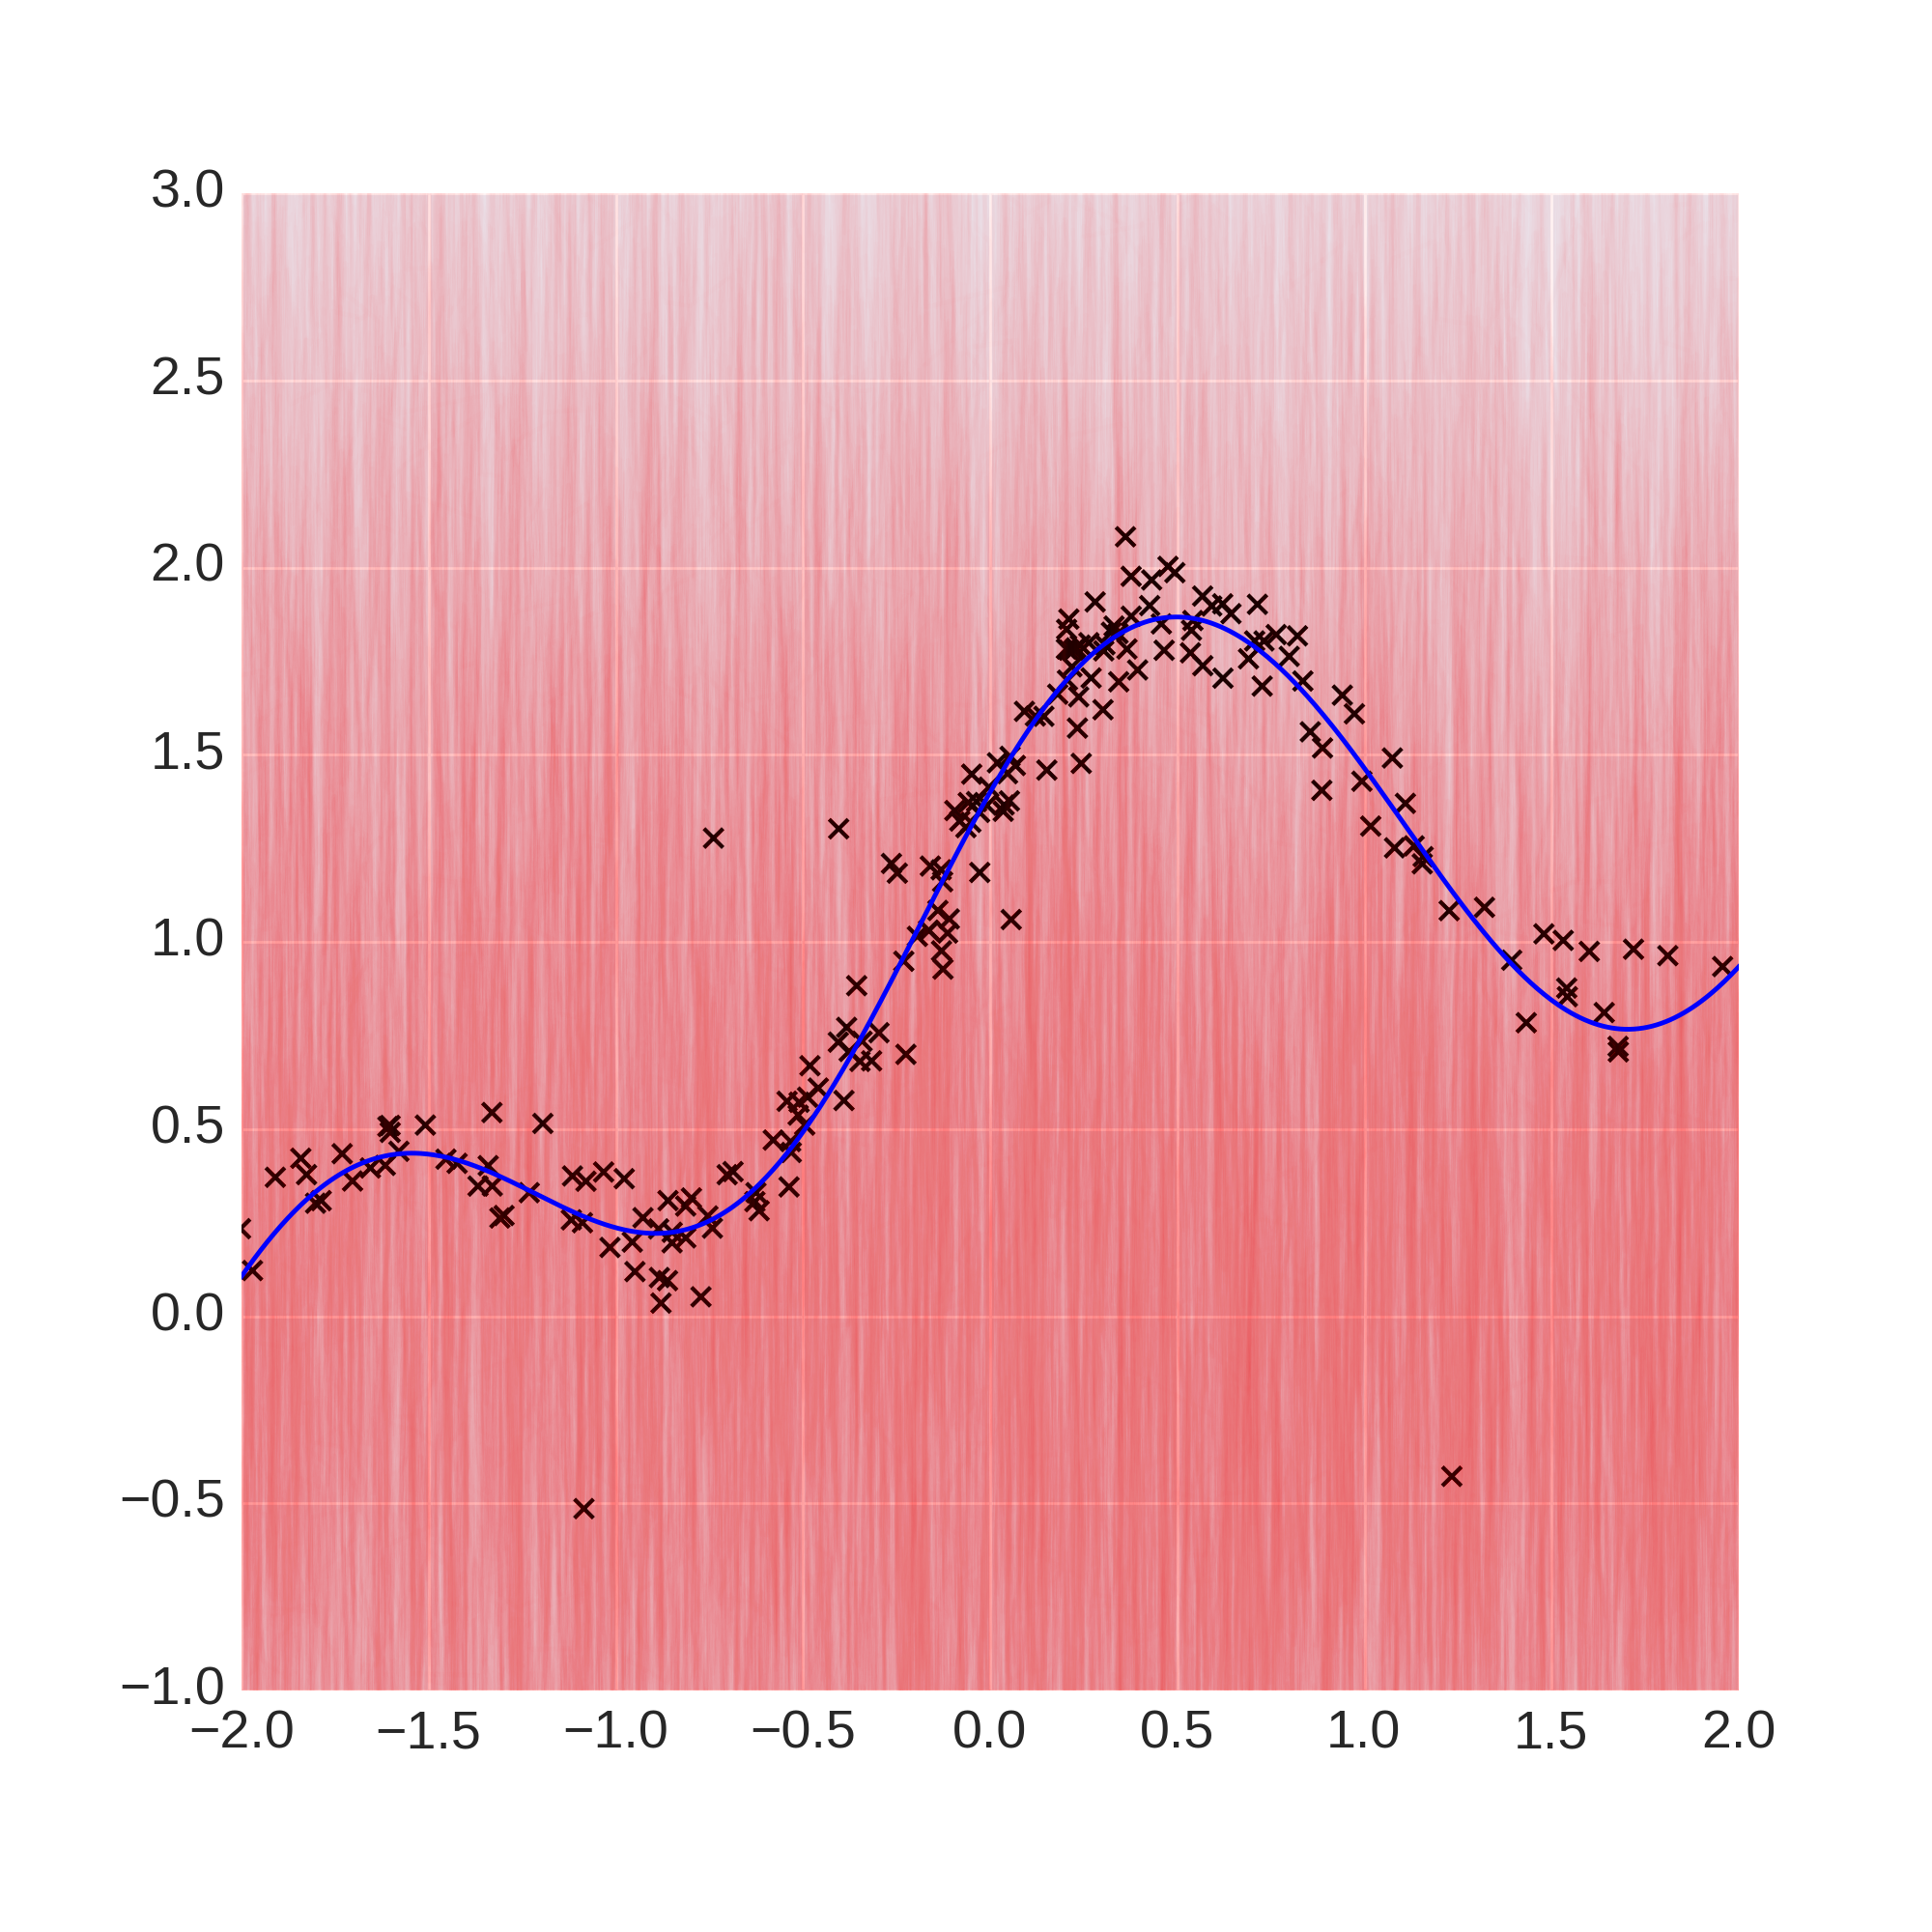
\includegraphics[height=7.5cm]{figs/neal_se_1final.png}
                \caption{Prior Inference}
                \label{fig:NealBO}
        \end{subfigure}%
        ~ %add desired spacing between images, e. g. ~, \quad, \qquad, \hfill etc.
          %(or a blank line to force the subfigure onto a new line)
          
        \begin{subfigure}[b]{0.49\textwidth} \centering
                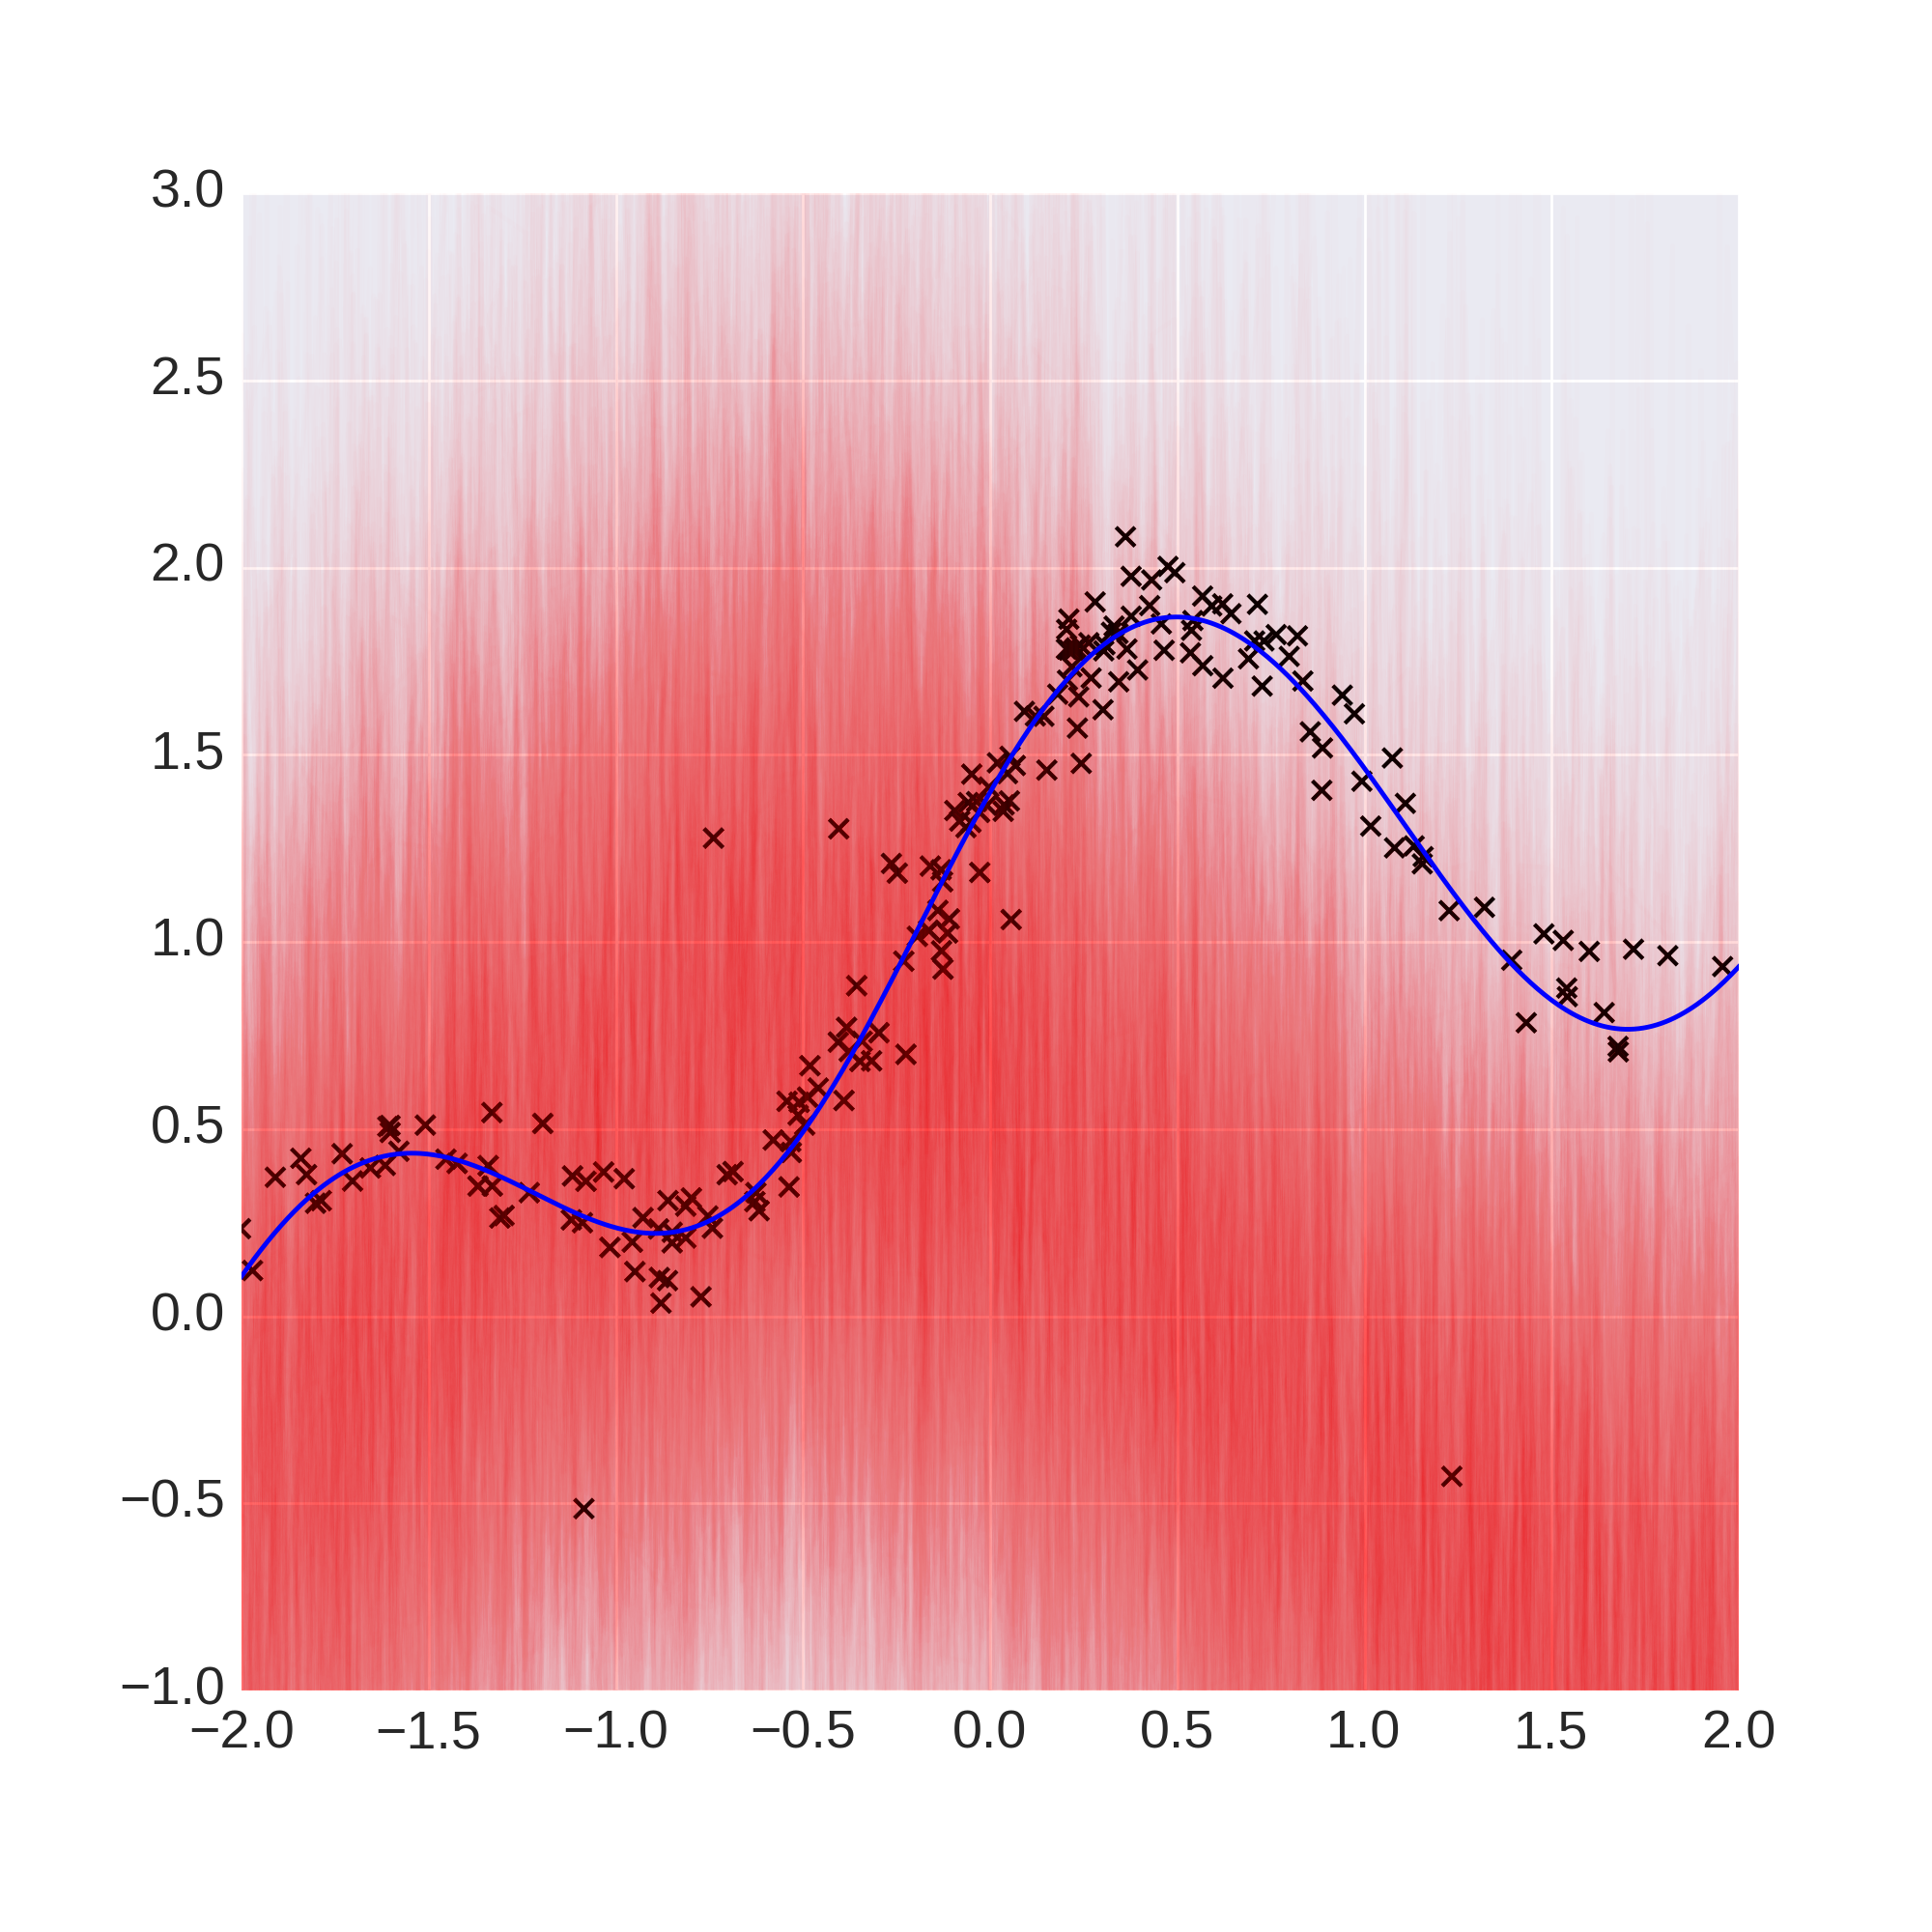
\includegraphics[height=7.5cm]{figs/neal_se_2final.png}
                \caption{Observed}
                \label{fig:NealAO}
        \end{subfigure}
        ~ %add desired spacing between images, e. g. ~, \quad, \qquad, \hfill etc.
          %(or a blank line to force the subfigure onto a new line)
        \begin{subfigure}[b]{0.49\textwidth} \centering
                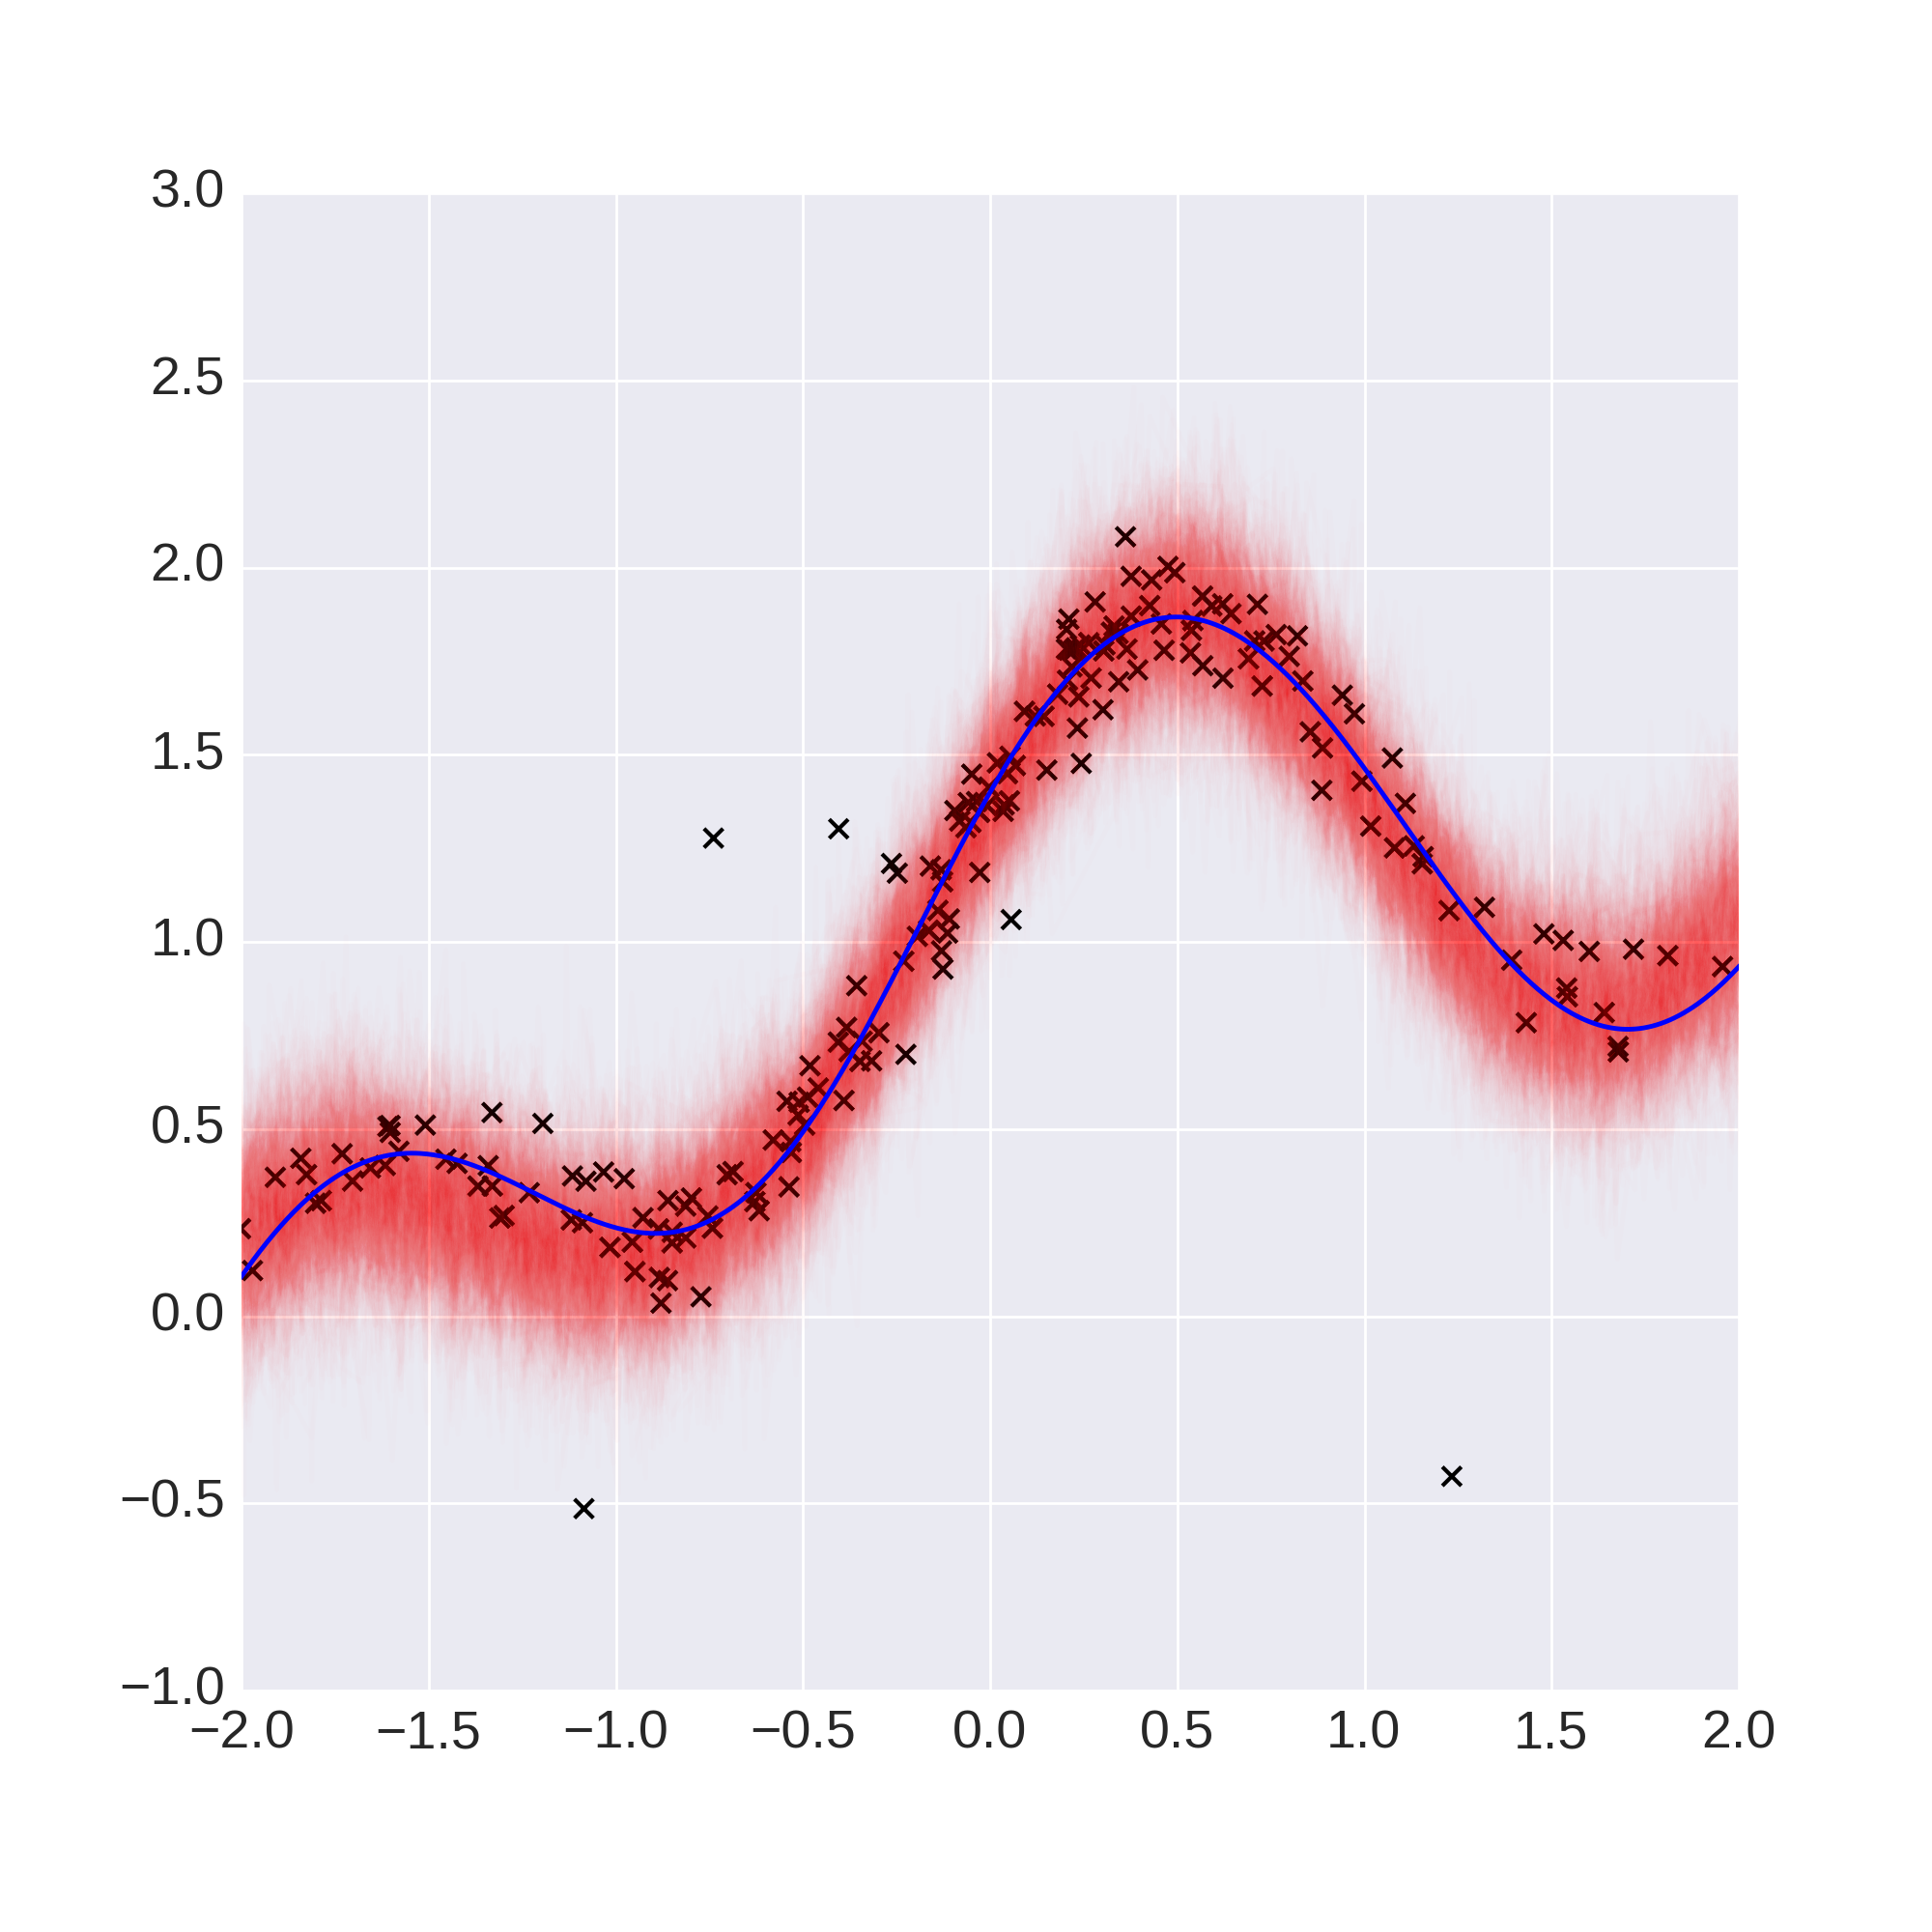
\includegraphics[height=7.5cm]{figs/neal_se_3final.png}
                \caption{Inferred}
                \label{fig:NealAI}
        \end{subfigure}
        \caption{(a) depicts the hierarchical structure of the hyper-parameter as constructed in the work by Neal as a Bayesian Network. (b)-(d) shows \gpmem\ on Neal's example. We see that prior renders functions all over the place (a). After \gpmem\ observes a some data-points an arbitrary smooth trend with a high level of noise is sampled. After running inference on the hierarchical system of hyper-parameters we see that the posterior reflects the actual curve well. Outliers are treated as such and do not confound the GP.}\label{fig:neal}
\end{figure}
We illustrate the hyper-parameter by showing the shift of the distribution on the noise parameter $\sigma$ (Fig. \ref{fig:inference}). We see that \gpmem\ learns the posterior distribution well, the posterior even exhibits a bimodal histogram when sampling $\sigma$ 100 times reflecting the two modes of data generation, that is normal noise and outliers\footnote{For this pedagogical example we have increased the probability for outliers in the data generation slightly from 0.05 to 0.2}. 

\begin{figure}
        \centering
        \begin{subfigure}[b]{0.5\textwidth} \centering
                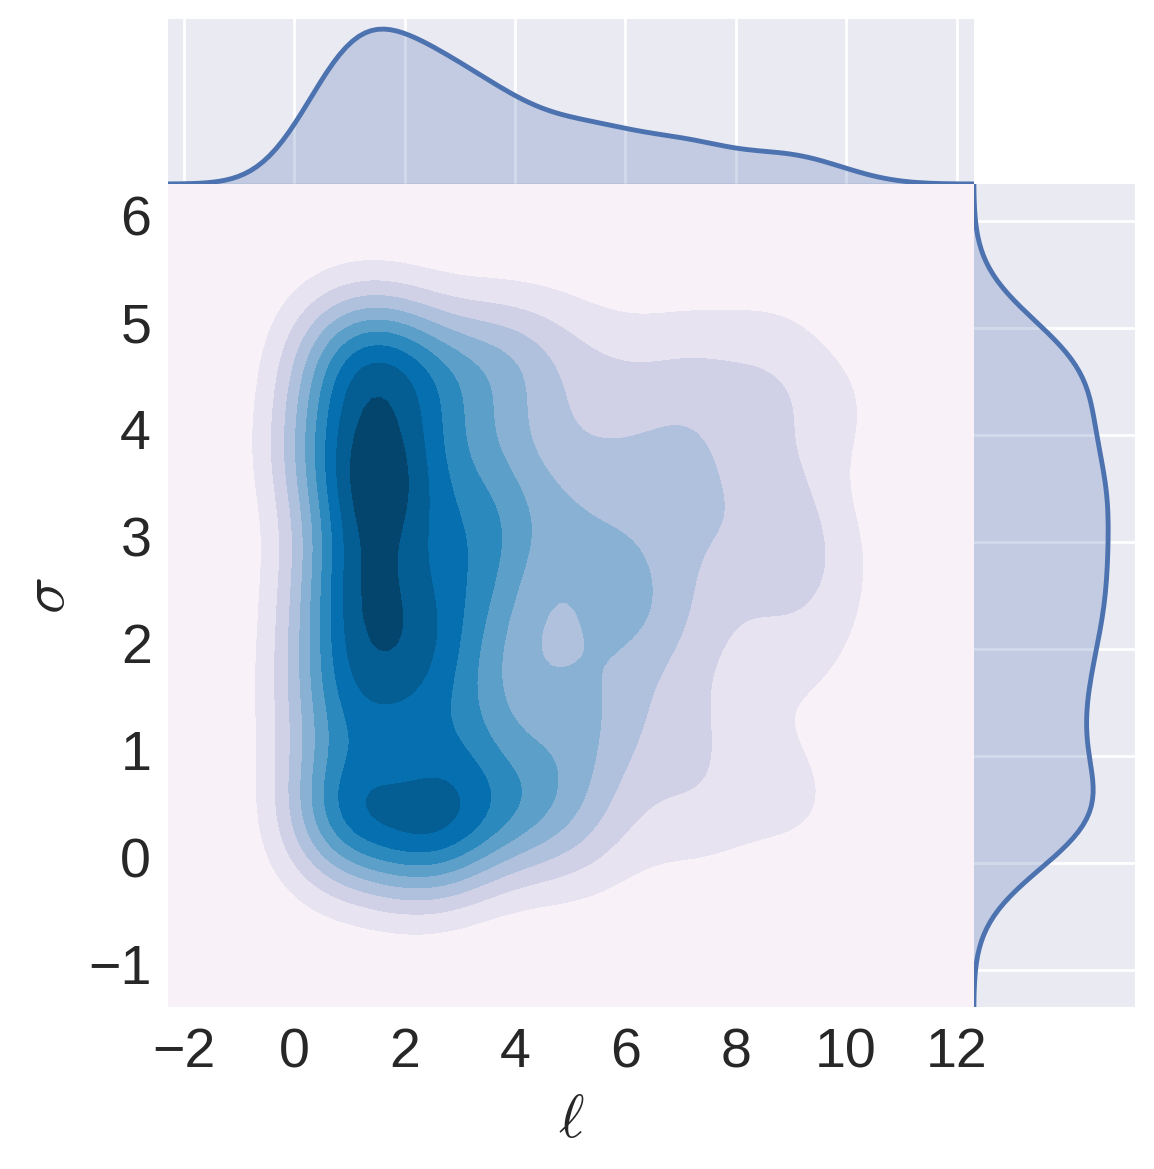
\includegraphics[height=6.5cm]{figs/neal_contour_l_vs_sigma_s__marginal_before.png}
                \caption{Before}
                \label{fig:before}
        \end{subfigure}%
        ~ %add desired spacing between images, e. g. ~, \quad, \qquad, \hfill etc.
          %(or a blank line to force the subfigure onto a new line)
        \begin{subfigure}[b]{0.5\textwidth} \centering
                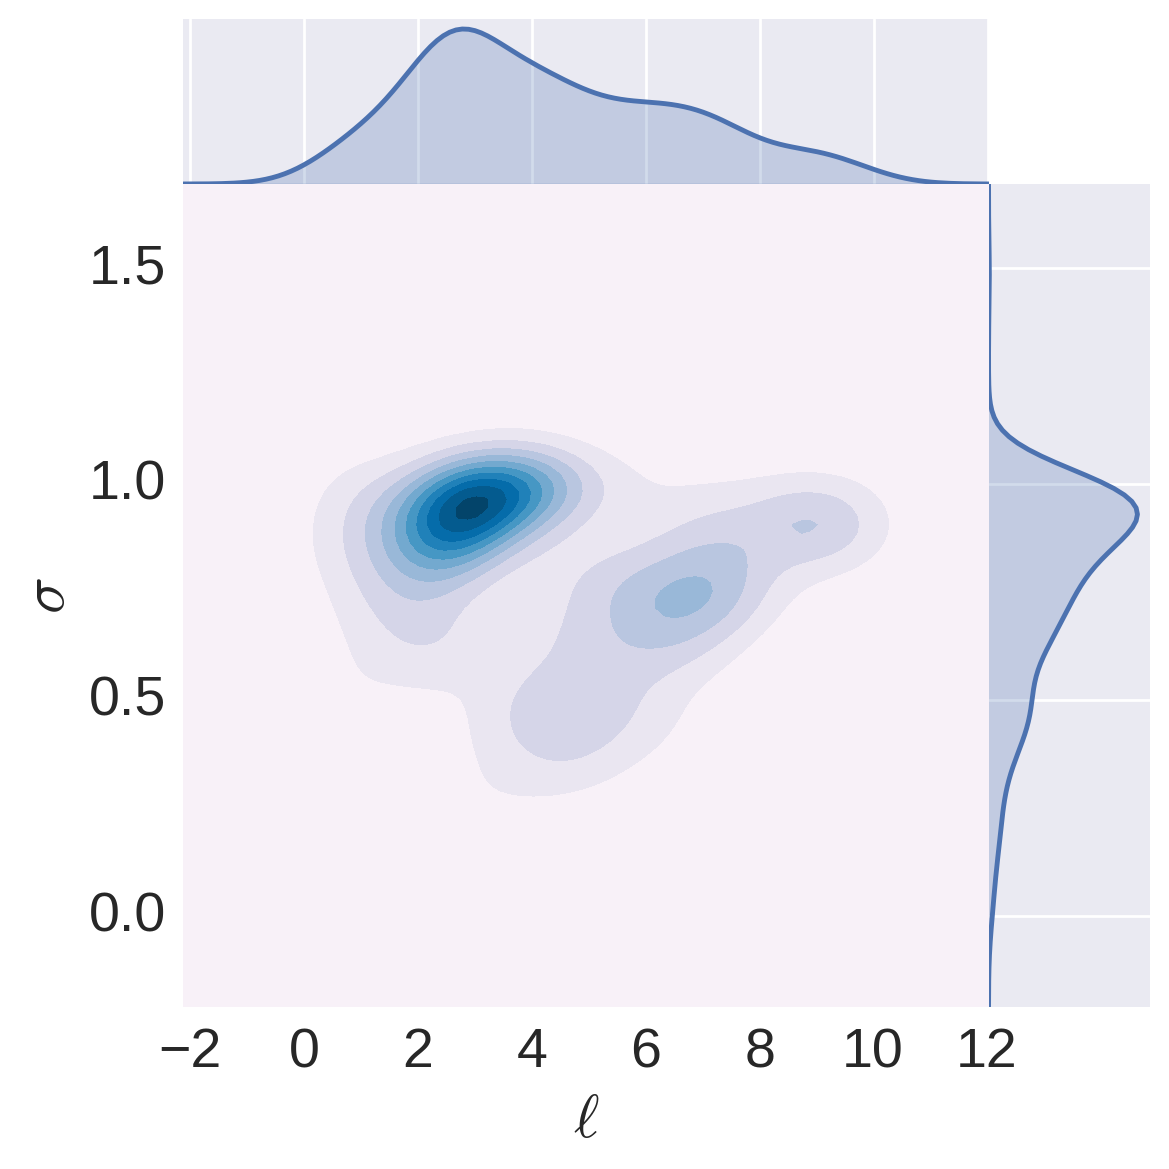
\includegraphics[height=6.5cm]{figs/neal_contour_l_vs_sigma_s__marginal_after.png}
                \caption{After}
                \label{fig:after))}
        \end{subfigure}
        \caption{Hyper-parameter inference on the parameter of the noise kernel. We show a 100 samples drawn from the distribution on $\sigma$. One can clearly recognise the shift from the uniform prior $\mathcal{U}(0,5)$ to a double peak distribution around the two modes - normal and outlier.}\label{fig:inference}
\end{figure}

